\documentclass[12pt,a4paper]{article}

% ---- Paketler ---------------------------------------------------------------
\usepackage[utf8]{inputenc}
\usepackage[T1]{fontenc}
\usepackage{geometry}
\geometry{margin=2.5cm, top=3cm}
\usepackage{graphicx}
\usepackage{booktabs}
\usepackage{array}
\usepackage{amsmath}
\usepackage[hidelinks]{hyperref}
\usepackage[dvipsnames,table]{xcolor}
\usepackage{titlesec}
\usepackage{enumitem}
\usepackage{fancyhdr}
\setlength{\headheight}{26pt}
\addtolength{\topmargin}{-14pt}
\usepackage{multirow}
\usepackage{float}
\usepackage{caption}
\usepackage{pgfplots}
\usepackage{tikz}
\usetikzlibrary{shapes.geometric, arrows.meta, positioning}
\pgfplotsset{compat=1.17}
\usepackage{tcolorbox}
\usepackage{setspace}
\onehalfspacing

% ---- Renk Tanimlari ---------------------------------------------------------
\definecolor{pblue}{RGB}{31,73,125}
\definecolor{ablue}{RGB}{68,114,196}
\definecolor{lgray}{RGB}{242,242,242}
\definecolor{dgray}{RGB}{64,64,64}
\definecolor{nred}{RGB}{198,40,40}

% ---- Baslik Bicimlendirmesi -------------------------------------------------
\titleformat{\section}
  {\large\bfseries\color{pblue}}{\thesection.}{0.5em}{}
  [\vspace{-0.5ex}\color{ablue}\rule{\linewidth}{0.6pt}]

\titleformat{\subsection}
  {\normalsize\bfseries\color{ablue}}{\thesubsection.}{0.5em}{}

\titleformat{\subsubsection}
  {\normalsize\itshape\color{dgray}}{\thesubsubsection.}{0.5em}{}

% ---- Ust/Alt Bilgi ----------------------------------------------------------
\pagestyle{fancy}
\fancyhf{}
\fancyhead[L]{\small\color{dgray}Veri Madenciliği Final Projesi}
\fancyhead[R]{\small\color{dgray}Pima Diyabetes Veri Seti Analizi}
\fancyfoot[C]{\thepage}
\renewcommand{\headrulewidth}{0.6pt}

% =============================================================================
\begin{document}

% ---- KAPAK SAYFASI ----------------------------------------------------------
\begin{titlepage}
  \centering
  \vspace*{1cm}

  {\Large\bfseries\color{pblue}İstanbul Gedik Üniversitesi\\[0.3em]
   \normalsize Mühendislik Fakültesi -- Bilgisayar Mühendisliği Bölümü}

  \vspace{1.5cm}
  {\color{pblue}\rule{\linewidth}{1.5pt}}\\[0.4em]
  {\huge\bfseries\color{pblue}
    Pima Diyabetes Veri Setinde\\[0.3em]
    Makine Öğrenmesi Algoritmalarının\\[0.3em]
    Karşılaştırmalı Analizi}\\[0.4em]
  {\color{pblue}\rule{\linewidth}{1.5pt}}

  \vspace{0.8cm}
  {\large\bfseries Veri Madenciliği -- Final Projesi}

  \vspace{1.2cm}
  \begin{tcolorbox}[
      colback=lgray,
      colframe=ablue,
      boxrule=1pt,
      arc=4pt,
      width=0.6\linewidth,
      halign=center
    ]
    \textbf{Hazırlayan}\\[0.4em]
    {\large Yahya Baltacı}\\[0.3em]
    Öğrenci No: 231041016\\[0.3em]
    Rol: Veri Mühendisi \& Model Mühendisi
  \end{tcolorbox}

  \vspace{0.8cm}
  \textbf{Danışman:} Dr. Mehmet Fatih Yüce\\[0.4em]
  \textbf{Ders Kodu:} BLM308

  \vspace{0.6cm}

% ---- BONUS TALEP LISTESI ------------------------------------------------
  \begin{tcolorbox}[
      colback=yellow!8,
      colframe=orange!70!black,
      boxrule=1pt,
      arc=4pt,
      width=0.85\linewidth
    ]
  {\bfseries\color{orange!70!black}Bonus Talepleri}\\[0.4em]
  \begin{tabular}{@{}lr@{}}
    LaTeX raporu + derlenmiş PDF teslimi & \textbf{+5 puan} \\[0.2em]
    GitHub deposu (açık, README ile) & \textbf{+5 puan} \\
    \multicolumn{2}{@{}l@{}}{\footnotesize\url{https://github.com/yahya308/verimadenciligifinal}} \\[0.2em]
    Demo videosu YouTube'a yüklendi (Liste Dışı) & \textbf{+5 puan} \\
    \multicolumn{2}{@{}l@{}}{\footnotesize\url{https://youtu.be/o6OsWhO8YJI}} \\[0.2em]
    Python ile Weka Karşılaştırması (\texttt{python\_karsilastirma.py}) & \textbf{+3 puan} \\[0.2em]
    Karmaşıklık Matrisleri üzerinden Tıbbi Hata Analizi (Rapor 7.2) & \textbf{+3 puan} \\[0.4em]
    \hline\\[-0.6em]
    \textit{Talep edilen toplam bonus} & \textit{\textbf{+21 puan}} \\
  \end{tabular}\\[0.3em]
  {\footnotesize Her kalem ayrı ayrı değerlendirilir; talep belirtilmeyen kalem puanlanmaz.}
  \end{tcolorbox}

  \vfill
  {\large\today}
\end{titlepage}

% ---- OZET -------------------------------------------------------------------
\begin{abstract}
\noindent
Bu çalışmada, Ulusal Diyabet, Sindirim ve Böbrek Hastalıkları Enstitüsü'nün
derlediği Pima Kızılderili Kadınları Diyabetes veri seti üzerinde üç farklı
makine öğrenmesi algoritmasının sınıflandırma performansı karşılaştırmalı olarak
incelenmiştir. Veri seti 768 örnek ve 8 klinik öznitelikten oluşmaktadır; hedef
değişken diyabet varlığını ikili olarak (pozitif/negatif) belirtmektedir.
CRISP-DM metodolojisi çerçevesinde gerçekleştirilen proje sürecinde; karar ağacı
(J48), olasılıksal (Naive Bayes) ve örnek tabanlı (IBk, $k{=}1$) sınıflandırıcılar,
10-katlı tabakalı çapraz doğrulama yöntemiyle değerlendirilmiştir. Doğruluk
açısından en yüksek performans \%76{,}30 ile Naive Bayes algoritmasında elde
edilmiş; bunu \%73{,}83 ile J48 ve \%70{,}18 ile IBk takip etmiştir. ROC-AUC
değeri de en yüksek Naive Bayes'te (0{,}819) gözlemlenmiş olup bu model klinik
karar destek sistemleri için en uygun aday olarak öne çıkmaktadır.
\end{abstract}

\newpage
\tableofcontents
\newpage

% =============================================================================
\section{Giriş ve Problem Tanımı}

\subsection{Motivasyon}

Diyabet, dünyada yaklaşık 537 milyon yetişkini etkileyen kronik bir metabolik
hastalık olup bu sayının 2045 yılına kadar 783 milyona ulaşması beklenmektedir
(IDF, 2021). Tip~2 diyabetin erken tespiti; kardiyovasküler komplikasyonları,
nöropatiyi ve organ yetmezliğini önleyebilmekte, tedavi maliyetlerini önemli
ölçüde düşürmektedir. Pima Kızılderili topluluğunun genetik ve yaşam tarzı
faktörleri nedeniyle yüksek diyabet prevalansına sahip olması, bu nüfusu
öngörüsel modellemelerde sık kullanılan bir referans haline getirmiştir.

Makine öğrenmesi yöntemleri, büyük hacimli ve çok değişkenli klinik verileri
işleyerek tanı destekleyici örüntüler çıkarmada geleneksel istatistiksel
yöntemlere göre çoğu zaman üstün performans sergilemektedir. Bu çalışmanın iş
değeri açısından çıktısı; klinik bütçesi kısıtlı ortamlarda (aile hekimlikleri,
sağlık ocakları) basit ölçümlerle yüksek riskli hastaları hızla tespit edebilecek
bir karar destek aracının teorik temelini oluşturmaktır.

\subsection{Araştırma Soruları}

\begin{enumerate}
  \item J48, Naive Bayes ve IBk algoritmaları Pima veri setinde birbirinden
        istatistiksel olarak anlamlı biçimde farklı performans göstermekte midir?
  \item Hangi klinik öznitelikler diyabeti en güçlü şekilde öngörmektedir?
  \item Seçilen en iyi model gerçek dünya klinik uygulaması için yeterince
        güvenilir midir?
\end{enumerate}

% =============================================================================
\section{Literatür Taraması}

Smith ve ark.\ (1988), orijinal ADAP öğrenme algoritmasını Pima veri setine
uygulamış ve \%76 doğruluk elde etmiştir; bu çalışma veri setinin temel
referansı olma özelliğini korumaktadır~\cite{smith1988using}.

Kavakiotis ve ark.\ (2017), diyabet tahmini üzerine yapılmış 85 makine öğrenmesi
çalışmasını meta-analiz yöntemiyle incelemiş; SVM ve rastgele ormanın en sık
kullanılan ve yüksek performanslı algoritmalar olduğunu saptamıştır. Pima veri
setindeki ortalama doğruluk değerinin \%74--80 bandında yoğunlaştığı
gözlemlenmiştir~\cite{kavakiotis2017machine}.

Sisodia ve Sisodia (2018), Naive Bayes, karar ağacı ve SVM'yi Pima veri seti
üzerinde karşılaştırmış; Naive Bayes'in \%76{,}30 doğrulukla rakiplerine göre
daha dengeli bir sınıflandırma sunduğunu raporlamıştır~\cite{sisodia2018prediction}.

Zou ve ark.\ (2018), derin öğrenme tabanlı bir model ile \%80{,}11 doğruluk
elde etmiş olmakla birlikte, küçük veri setlerinde aşırı öğrenme riskine
dikkat çekmiştir~\cite{zou2018predicting}.

Khourdifi ve Bahaj (2019), birleşik öznitelik seçimi ve topluluk öğrenmesi
yöntemleriyle Pima veri setinde \%82'ye varan doğruluk bildirmiştir; bu
sonuçlar ön işleme ve öznitelik mühendisliğinin kritik rolünü
vurgulamaktadır~\cite{khourdifi2019heart}.

% =============================================================================
\section{CRISP-DM Metodolojisi}

Bu proje, Çapraz Endüstri Veri Madenciliği Standart Süreci (CRISP-DM)
çerçevesinde altı aşama olarak yürütülmüştür. Şekil~\ref{fig:crispdm} söz konusu
aşamaları özetlemektedir.

\begin{figure}[H]
\centering
\begin{tikzpicture}[node distance=1.4cm,
  box/.style={
    rectangle, rounded corners=5pt,
    draw=ablue, fill=lgray,
    text width=2.2cm, align=center,
    font=\small\bfseries, minimum height=0.85cm
  },
  arr/.style={-Stealth, thick, draw=ablue}
]
  \node[box] (bu) {İş Anlayışı};
  \node[box, right=of bu] (du) {Veri Anlayışı};
  \node[box, right=of du] (dp) {Veri Ön İşleme};
  \node[box, right=of dp] (mo) {Modelleme};
  \node[box, right=of mo] (ev) {Değerlendirme};
  \node[box, right=of ev] (de) {Yayılım};

  \draw[arr] (bu) -- (du);
  \draw[arr] (du) -- (dp);
  \draw[arr] (dp) -- (mo);
  \draw[arr] (mo) -- (ev);
  \draw[arr] (ev) -- (de);

  \draw[arr, bend left=45] (du) to (bu);
  \draw[arr, bend left=45] (ev) to (mo);
  \draw[arr, bend left=55] (ev) to (bu);
\end{tikzpicture}
\caption{CRISP-DM süreç akışı ve iteratif adımlar}
\label{fig:crispdm}
\end{figure}

% =============================================================================
\section{Veri Tanımı ve Keşifsel Veri Analizi}

\subsection{Veri Kaynağı ve Tanımı}

Veri seti, UCI Makine Öğrenmesi Deposu'nda ve Kaggle'da yaygın biçimde
erişilebilen \textit{Pima Indians Diabetes Database} olup
Tablo~\ref{tab:dataset}'de temel özellikleri sunulmaktadır.

\begin{table}[H]
\centering
\caption{Veri seti özeti}
\label{tab:dataset}
\begin{tabular}{@{}ll@{}}
\toprule
\textbf{Özellik} & \textbf{Değer} \\
\midrule
Kaynak & UCI / NIDDK \\
Örnek sayısı & 768 \\
Öznitelik sayısı & 8 (sayısal) + 1 sınıf \\
Sınıf dağılımı & \texttt{tested\_negative}: 500 (\%65{,}1) \\
               & \texttt{tested\_positive}: 268 (\%34{,}9) \\
Eksik değer & Biyolojik 0-değerler eksik veriyi temsil eder \\
\bottomrule
\end{tabular}
\end{table}

\begin{table}[H]
\centering
\caption{Öznitelik açıklamaları}
\label{tab:features}
\begin{tabular}{@{}lll@{}}
\toprule
\textbf{Öznitelik} & \textbf{Açıklama} & \textbf{Birim} \\
\midrule
\texttt{preg}  & Hamilelik sayısı                        & adet \\
\texttt{plas}  & 2 saatlik oral glikoz tolerans testi    & mg/dL \\
\texttt{pres}  & Diyastolik kan basıncı                  & mm~Hg \\
\texttt{skin}  & Triceps deri kıvrımı kalınlığı          & mm \\
\texttt{insu}  & 2 saatlik serum insülini                & $\mu$U/mL \\
\texttt{mass}  & Vücut kitle indeksi (VKİ)               & kg/m$^{2}$ \\
\texttt{pedi}  & Diyabet soyağacı fonksiyonu             & -- \\
\texttt{age}   & Yaş                                     & yıl \\
\texttt{class} & Hedef: diyabet durumu                   & ikili \\
\bottomrule
\end{tabular}
\end{table}

\subsection{Sınıf Dağılımı}

Veri setinde sınıf dengesi oranının yaklaşık 1{,}87:1 (negatif:pozitif)
olduğu görülmektedir (bkz. Şekil~\ref{fig:classdist}). Bu hafif dengesizlik,
pozitif sınıfın geri çağırma (recall) değerlerinin negatif sınıfa göre
sistematik olarak düşük kalmasına yol açmaktadır.

\begin{figure}[H]
\centering
\begin{tikzpicture}
\begin{axis}[
  ybar,
  bar width=1.4cm,
  symbolic x coords={Negatif (500), Pozitif (268)},
  xtick=data,
  ymin=0, ymax=600,
  ylabel={Örnek Sayısı},
  nodes near coords,
  nodes near coords align=vertical,
  every node near coord/.append style={font=\small},
  width=9cm, height=6.5cm,
  enlarge x limits=0.5,
  title={Sınıf Dağılımı ($n{=}768$)},
  title style={font=\bfseries}
]
  \addplot[fill=ablue!70, draw=pblue] coordinates {(Negatif (500),500)};
  \addplot[fill=nred!65,  draw=nred]  coordinates {(Pozitif (268),268)};
\end{axis}
\end{tikzpicture}
\caption{Hedef sınıfların dağılımı}
\label{fig:classdist}
\end{figure}

\subsection{Öznitelik Ortalamaları: Sınıfa Göre Karşılaştırma}

Tablo~\ref{tab:means}, Naive Bayes modelinin öğrendiği sınıf koşullu
ortalamalardan elde edilen karşılaştırmalı istatistikleri göstermektedir.

\begin{table}[H]
\centering
\caption{Özniteliklerin sınıfa göre ortalama değerleri (Naive Bayes çıktısından)}
\label{tab:means}
\begin{tabular}{@{}lrrr@{}}
\toprule
\textbf{Öznitelik} &
\textbf{Negatif (Ort.)} &
\textbf{Pozitif (Ort.)} &
\textbf{Fark} \\
\midrule
\texttt{preg}  & 3{,}42   & 4{,}98   & +1{,}56 \\
\texttt{plas}  & 109{,}95 & 141{,}26 & \textbf{+31{,}31} \\
\texttt{pres}  & 68{,}14  & 70{,}72  & +2{,}58 \\
\texttt{skin}  & 19{,}84  & 22{,}28  & +2{,}44 \\
\texttt{insu}  & 68{,}85  & 100{,}28 & +31{,}43 \\
\texttt{mass}  & 30{,}30  & 35{,}15  & \textbf{+4{,}85} \\
\texttt{pedi}  & 0{,}430  & 0{,}550  & +0{,}120 \\
\texttt{age}   & 31{,}25  & 37{,}08  & +5{,}83 \\
\bottomrule
\end{tabular}
\end{table}

En büyük mutlak fark \texttt{plas} (plazma glikozu) ve \texttt{insu}
özniteliklerinde gözlemlenmektedir. Bu durum, karar ağacı modelinin birincil
ayrım noktası olarak \texttt{plas} $\leq 127$ eşiğini kullanmasıyla uyum
içindedir.

\subsection{Öznitelik Önem Sıralaması}

\begin{figure}[H]
\centering
\begin{tikzpicture}
\begin{axis}[
  xbar,
  bar width=0.42cm,
  symbolic y coords={preg, pres, pedi, skin, insu, age, mass, plas},
  ytick=data,
  xlabel={Göreceli Önem (J48 ağaç yapısına göre)},
  xmin=0, xmax=10,
  nodes near coords,
  nodes near coords align=horizontal,
  every node near coord/.append style={font=\scriptsize},
  width=11cm, height=7cm,
  title={Öznitelik Önemi -- J48 Ağaç Yapısı},
  title style={font=\bfseries}
]
  \addplot[fill=ablue!80, draw=pblue] coordinates {
    (3,preg)(2,pres)(5,pedi)(2,skin)(2,insu)(4,age)(6,mass)(9,plas)
  };
\end{axis}
\end{tikzpicture}
\caption{J48 karar ağacındaki dallanma yapısına dayalı öznitelik önem skoru}
\label{fig:featimp}
\end{figure}

% =============================================================================
\section{Veri Ön İşleme}
\label{sec:preproc}

\subsection{Biyolojik Açıdan Geçersiz Sıfır Değerler}

\texttt{plas}, \texttt{pres}, \texttt{skin}, \texttt{insu} ve \texttt{mass}
özniteliklerindeki 0 değerleri biyolojik olarak anlamsızdır (sıfır kan basıncı
veya sıfır VKİ mümkün değildir). Bu değerler aslında eksik ölçümleri temsil
etmektedir. Bu çalışmada ham veri WEKA'ya aktarılarak sınıflandırıcıların
varsayılan davranışı gözlemlenmiştir.

\subsection{Ölçek Farklılıkları ve Normalizasyon}

Öznitelikler birbirinden farklı ölçek aralığına sahiptir
(örneğin \texttt{insu}: 0--846, \texttt{pedi}: 0{,}08--2{,}42).
Mesafeye duyarlı IBk algoritması için MinMax veya $z$-skor normalizasyonu
kritik öneme sahiptir. WEKA'nın \texttt{EuclideanDistance -R first-last}
parametresi tüm öznitelik aralığını kapsamakla birlikte, ölçek farklılıkları
giderilmediği sürece mesafe hesabı yanlı kalabilmektedir.

\subsection{Sınıf Dengesizliği}

Negatif:pozitif oranı 1{,}87:1 seviyesindedir. Gelecek çalışmalarda SMOTE
veya ağırlıklı örnekleme ile bu durum giderilebilir.

% =============================================================================
\section{Modelleme}

\subsection{Seçilen Algoritmalar ve Gerekçeler}

\paragraph{J48 (C4.5 Karar Ağacı)}
Quinlan'ın C4.5 algoritmasının WEKA uyarlaması olan J48, bilgi kazancı oranına
dayalı dallanma ve hata tabanlı budama (\texttt{-C~0.25}, min. yaprak $=2$) ile
yorumlanabilir bir karar ağacı üretir. Hem görsel yorumlanabilirlik hem de
tıbbi karar kurallarına doğrudan çevrilebilir yapısı nedeniyle seçilmiştir.

\paragraph{Naive Bayes}
Öznitelik bağımsızlığı varsayımı altında Bayes teoremini uygulayan bu
sınıflandırıcı, sürekli öznitelikler için Gaussian dağılım kullanır.
Hesapsal verimliliği, küçük-orta ölçekli medikal veri setlerindeki güçlü
performansı ve düşük varyans riski nedeniyle tercih edilmiştir.

\paragraph{IBk ($k{=}1$, k-En Yakın Komşu)}
En yaygın instance-based öğrenme modeli olan 1-NN, eğitim verisini doğrudan
bellek olarak kullanır. Karmaşık karar sınırlarını parametresiz öğrenebilmesi
avantajıyla seçilmiş; ancak gürültüye duyarlılığı nedeniyle en düşük
genelleme performansına sahip algoritma olarak konumlandırılmıştır.

\subsection{Deney Kurulumu}

\begin{tcolorbox}[colback=lgray, colframe=ablue,
                  title={\bfseries\color{white}Değerlendirme Protokolü}]
\begin{itemize}[leftmargin=*]
  \item \textbf{Yöntem:} 10-katlı tabakalı çapraz doğrulama
  \item \textbf{Araç:} WEKA 3.x -- Explorer arayüzü
  \item \textbf{Metrikler:} Doğruluk, Kappa, F-Measure, ROC-AUC, PRC-AUC
  \item \textbf{Parametreler:} J48: $C{=}0{,}25$, $M{=}2$; Naive Bayes: Gaussian; IBk: $k{=}1$, Öklid mesafesi
\end{itemize}
\end{tcolorbox}

% =============================================================================
\section{Performans Değerlendirmesi}

\subsection{Genel Karşılaştırma Tablosu}

\begin{table}[H]
\centering
\caption{Algoritmaların 10-katlı çapraz doğrulama sonuçları}
\label{tab:results}
\begin{tabular}{@{}lrrrrrrr@{}}
\toprule
\textbf{Algoritma} &
\textbf{Doğr.\%} &
\textbf{Kappa} &
\textbf{MAE} &
\textbf{RMSE} &
\textbf{F1} &
\textbf{ROC} &
\textbf{PRC} \\
\midrule
J48             & 73{,}83 & 0{,}416 & 0{,}316 & 0{,}446 & 0{,}736 & 0{,}751 & 0{,}727 \\
\rowcolor{ablue!15}
Naive Bayes     & \textbf{76{,}30} & \textbf{0{,}466} & \textbf{0{,}284} & \textbf{0{,}417} & \textbf{0{,}760} & \textbf{0{,}819} & \textbf{0{,}815} \\
IBk ($k{=}1$)  & 70{,}18 & 0{,}330 & 0{,}299 & 0{,}545 & 0{,}698 & 0{,}650 & 0{,}640 \\
\bottomrule
\end{tabular}
\end{table}

Tüm metriklerde \textbf{Naive Bayes} en yüksek performansı sergilemiştir.
ROC-AUC değerinin 0{,}819 olması, modelin eşik değerinden bağımsız olarak
güçlü bir ayrım kapasitesine sahip olduğunu göstermektedir.

\subsection{Karmaşıklık Matrisleri}

\begin{table}[H]
\centering
\caption{Karmaşıklık matrisleri -- tahmin edilen sınıf (sütun) ve gerçek sınıf (satır)}
\label{tab:confusion}
\begin{tabular}{@{}l cc cc cc@{}}
\toprule
& \multicolumn{2}{c}{\textbf{J48}}
& \multicolumn{2}{c}{\textbf{Naive Bayes}}
& \multicolumn{2}{c}{\textbf{IBk ($k{=}1$)}} \\
\cmidrule(lr){2-3}\cmidrule(lr){4-5}\cmidrule(lr){6-7}
\textbf{Gerçek~/~Tahmin} &
\textbf{Neg.} & \textbf{Poz.} &
\textbf{Neg.} & \textbf{Poz.} &
\textbf{Neg.} & \textbf{Poz.} \\
\midrule
tested\_negative (500) & 407 &  93 & 422 &  78 & 397 & 103 \\
tested\_positive  (268) & 108 & 160 & 104 & 164 & 126 & 142 \\
\midrule
Yanlış Negatif (FN) & \multicolumn{2}{c}{108}
                    & \multicolumn{2}{c}{\textbf{104}}
                    & \multicolumn{2}{c}{126} \\
Yanlış Pozitif (FP) & \multicolumn{2}{c}{93}
                    & \multicolumn{2}{c}{\textbf{78}}
                    & \multicolumn{2}{c}{103} \\
\bottomrule
\end{tabular}
\end{table}

\textbf{Klinik Yorum:} Medikal tanı uygulamalarında yanlış negatif (FN)
-- yani hasta olduğu halde sağlıklı sınıflandırılan bireyler -- yanlış
pozitiften çok daha maliyetlidir. Bu açıdan \textbf{Naive Bayes}, 104 FN
ile en düşük kaçırma oranını sergilemiş ve klinik güvenlik açısından öne
çıkmıştır.

\subsection{Sınıfa Göre Detaylı Performans}

\begin{table}[H]
\centering
\caption{Sınıf bazında Kesinlik, Geri Çağırma ve F-Measure değerleri}
\label{tab:classperf}
\begin{tabular}{@{}llrrrr@{}}
\toprule
\textbf{Algoritma} & \textbf{Sınıf} &
\textbf{Kesinlik} & \textbf{GÇ} & \textbf{F1} & \textbf{ROC-AUC} \\
\midrule
\multirow{2}{*}{J48}
  & tested\_negative & 0{,}790 & 0{,}814 & 0{,}802 & 0{,}751 \\
  & tested\_positive & 0{,}632 & 0{,}597 & 0{,}614 & 0{,}751 \\
\midrule
\multirow{2}{*}{Naive Bayes}
  & tested\_negative & 0{,}802 & 0{,}844 & \textbf{0{,}823} & \textbf{0{,}819} \\
  & tested\_positive & 0{,}678 & 0{,}612 & \textbf{0{,}643} & \textbf{0{,}819} \\
\midrule
\multirow{2}{*}{IBk ($k{=}1$)}
  & tested\_negative & 0{,}759 & 0{,}794 & 0{,}776 & 0{,}650 \\
  & tested\_positive & 0{,}580 & 0{,}530 & 0{,}554 & 0{,}650 \\
\bottomrule
\end{tabular}
\end{table}

\subsection{Bias-Variance Analizi}

\begin{table}[H]
\centering
\caption{Algoritmaların bias-variance değerlendirmesi}
\label{tab:biasvar}
\begin{tabular}{@{}lp{5.2cm}p{5.2cm}@{}}
\toprule
\textbf{Algoritma} & \textbf{Bias Durumu} & \textbf{Variance Durumu} \\
\midrule
J48 &
  Orta bias: budama gereksiz dallanmayı engeller; eğitim doğruluğu teste göre
  belirgin şekilde yüksektir. &
  Orta variance: ağaç yapısı verideki gürültüye kısmen duyarlıdır. \\
\midrule
Naive Bayes &
  Yüksek bias: bağımsızlık ve Gaussian varsayımları gerçek ilişkileri
  basitleştirir; ancak bu veri setine görece iyi uymaktadır. &
  Düşük variance: parametre sayısı azdır, overfitting riski düşüktür. \\
\midrule
IBk ($k{=}1$) &
  Çok düşük bias: eğitim verisini ezberler. &
  Çok yüksek variance: test doğruluğu \%70{,}18'e düşmektedir;
  gürültüye son derece duyarlıdır. \\
\bottomrule
\end{tabular}
\end{table}

\subsection{Python (scikit-learn) ve WEKA Karşılaştırması (Ek Çalışma)}

WEKA ortamında elde edilen sonuçların tutarlılığını bağımsız bir kütüphane ile doğrulamak amacıyla, en yüksek performansı gösteren Naive Bayes modeli Python \texttt{scikit-learn} kütüphanesi kullanılarak yeniden modellenmiştir. Tıpkı WEKA'da olduğu gibi veriler 10-katlı tabakalı çapraz doğrulama (Stratified 10-Fold CV) yöntemiyle test edilmiş ve aşağıdaki sonuçlar elde edilmiştir:

\begin{itemize}
  \item \textbf{WEKA Sonuçları:} Doğruluk: \%76{,}30, ROC-AUC: 0{,}819
  \item \textbf{Python Sonuçları:} Doğruluk: \%75{,}52, ROC-AUC: 0{,}814
\end{itemize}

\textbf{Değerlendirme:} İki farklı geliştirme ortamı arasındaki yaklaşık \%0{,}78'lik bu ufak fark literatürde beklenen, doğal bir durumdur. Bu sapmanın temel nedeni; çapraz doğrulama sırasında verilerin rastgele 10 parçaya bölünürken kullanılan karıştırma (shuffling) algoritmalarının farklılıkları ve her iki kütüphanenin alt seviyedeki kayan nokta (floating-point) hassasiyeti hesaplamalarındaki mikro değişikliklerdir. Python üzerinden alınan bu sonuçlar, WEKA analizlerimizi güçlü bir şekilde doğrulamakta ve modelin tutarlılığını kanıtlamaktadır.

% =============================================================================
\section{J48 Karar Ağacı Yorumu}

WEKA'nın ürettiği J48 ağacı \textbf{20 yaprak} ve \textbf{39 düğüm}e sahiptir.
Ağacın kök bölünme özniteliği \texttt{plas} $\leq 127$'dir; bu plazma
glikozunun birincil ayırt edici öznitelik olduğunu doğrulamaktadır.
İkincil ayrım noktaları şunlardır:

\begin{itemize}
  \item \texttt{mass} $\leq 26{,}4$: düşük VKİ durumunda negatif sınıfı güçlü
        biçimde işaret eder (132 örnek, yalnızca 3 hata).
  \item \texttt{age} $\leq 28$: genç bireyler için ek negatif göstergesi.
  \item \texttt{pedi} $> 0{,}56$ ve \texttt{preg} $> 6$: yüksek soyağacı skoru
        ve çok sayıda hamilelik, pozitif sınıfı güçlendiren kuraldır.
  \item \texttt{plas} $> 157$: derin sağ dalda güçlü pozitif göstergesi
        (92 örnek, 12 hata).
\end{itemize}

Bu kurallar, klinisyenlerin kolayca yorumlayabileceği beyaz-kutu bir karar
destek yapısı sunmaktadır.

% =============================================================================
\section{Sonuç ve Tartışma}

\subsection{Temel Bulgular}

Bu çalışmada Pima Diyabetes veri seti üzerinde üç farklı makine öğrenmesi
algoritması 10-katlı çapraz doğrulama ile değerlendirilmiştir.
Elde edilen başlıca bulgular şunlardır:

\begin{enumerate}
  \item \textbf{Naive Bayes en başarılı modeldir.} \%76{,}30 doğruluk,
        0{,}819 ROC-AUC ve en düşük yanlış negatif sayısı (104) ile klinik
        tercih kriterlerini en iyi karşılayan algoritma olmuştur.
  \item \textbf{Plazma glikozu (\texttt{plas}) baskın özniteliktir.}
        Hem karar ağacı yapısında hem de sınıflar arası ortalama farklarında
        belirleyici şekilde öne çıkmaktadır.
  \item \textbf{IBk ($k{=}1$) aşırı öğrenme nedeniyle en zayıf genellemeyi
        sergilemiştir.} $k$ değeri artırılarak ve öznitelik normalizasyonu
        uygulanarak performans iyileştirilebilir.
\end{enumerate}

\subsection{Kısıtlar}

\begin{itemize}
  \item Veri setinin yalnızca Pima Kızılderili kadınlarını kapsaması
        genelleştirilme gücünü azaltmaktadır.
  \item Sıfır değerlerin sistematik bir imputation yöntemiyle işlenmemesi
        model kalitesini olumsuz etkileyebilir.
  \item Hiperparametre optimizasyonu yapılmamıştır.
\end{itemize}

\subsection{Gelecek Çalışmalar}

\begin{itemize}
  \item SMOTE ile sınıf dengesizliğinin giderilmesi.
  \item Grid-search ile hiperparametre ayarı; SVM ve Random Forest gibi
        güçlü sınıflandırıcıların eklenmesi.
  \item Öznitelik seçimi (wrapper/filter) ile boyut indirgeme.
  \item Farklı popülasyonlarda dış doğrulama.
\end{itemize}

% =============================================================================
\newpage
\begin{thebibliography}{9}

\bibitem{smith1988using}
Smith, J.~W., Everhart, J.~E., Dickson, W.~C., Knowler, W.~C., \& Johannes, R.~S. (1988).
Using the ADAP learning algorithm to forecast the onset of diabetes mellitus.
\textit{Proceedings of the Annual Symposium on Computer Application in Medical Care}, 261--265.

\bibitem{kavakiotis2017machine}
Kavakiotis, I., Tsave, O., Salifoglou, A., Maglaveras, N., Vlahavas, I., \& Chouvarda, I. (2017).
Machine learning and data mining methods in diabetes research.
\textit{Computational and Structural Biotechnology Journal}, 15, 104--116.

\bibitem{sisodia2018prediction}
Sisodia, D., \& Sisodia, D.~S. (2018).
Prediction of diabetes using classification algorithms.
\textit{Procedia Computer Science}, 132, 1578--1585.

\bibitem{zou2018predicting}
Zou, Q., Qu, K., Luo, Y., Yin, D., Ju, Y., \& Tang, H. (2018).
Predicting diabetes mellitus with machine learning techniques.
\textit{Frontiers in Genetics}, 9, 515.

\bibitem{khourdifi2019heart}
Khourdifi, Y., \& Bahaj, M. (2019).
Heart disease prediction and classification using machine learning algorithms
optimized by particle swarm optimization and ant colony optimization.
\textit{International Journal of Intelligent Engineering and Systems}, 12(1), 242--252.

\bibitem{uci2022pima}
Dua, D., \& Graff, C. (2019).
\textit{UCI Machine Learning Repository -- Pima Indians Diabetes Database}.
University of California, Irvine.
\url{https://archive.ics.uci.edu/ml/datasets/diabetes}

\bibitem{witten2016data}
Witten, I.~H., Frank, E., Hall, M.~A., \& Pal, C.~J. (2016).
\textit{Data Mining: Practical Machine Learning Tools and Techniques} (4.~baskı).
Morgan Kaufmann.

\bibitem{han2011data}
Han, J., Kamber, M., \& Pei, J. (2011).
\textit{Data Mining: Concepts and Techniques} (3.~baskı).
Morgan Kaufmann.

\end{thebibliography}

% =============================================================================
\newpage
\section*{Yapay Zeka Kullanım Beyanı}

Bu proje kapsamında aşağıda belirtilen yapay zeka aracından yararlanılmıştır:

\begin{itemize}
  \item \textbf{Gemini (Google):} LaTeX rapor şablonu oluşturma,
        bölümlerin yazım düzenlenmesi ve biçimlendirilmesi amacıyla kullanılmıştır.
\end{itemize}

Projenin aşağıda belirtilen tüm aşamaları tamamen öğrenci tarafından
gerçekleştirilmiştir:

\begin{itemize}
  \item Problem tanımı ve araştırma sorularının belirlenmesi
  \item WEKA ortamında J48, Naive Bayes ve IBk algoritmalarının çalıştırılması
  \item 10-katlı çapraz doğrulama deney kurulumu ve parametrelerinin seçimi
  \item Çıktı verisinin yorumlanması ve karşılaştırmalı analiz
  \item Sonuçların klinik açıdan değerlendirilmesi
\end{itemize}

Yönerge gereğince tüm yapay zeka kullanımı bu bölümde beyan edilmiştir.

% =============================================================================
\section*{Proje Deposu}

Projenin tüm kaynak kodları, veri seti, WEKA çıktıları ve bu rapor aşağıdaki
GitHub deposunda açık kaynak olarak yayınlanmıştır:

\begin{center}
  \url{https://github.com/yahya308/verimadenciligifinal}
\end{center}

Depoda bulunan dosyalar: \texttt{main.tex}, \texttt{verimadenciligi.pdf},
\texttt{diabetes.arff}, \texttt{j48.txt}, \texttt{NaiveBayes.txt},
\texttt{IBK.txt}, \texttt{sunumvideo.mp4}, \texttt{README.txt}, \texttt{python\_karsilastirma.py}.

\end{document}